% Options for packages loaded elsewhere
\PassOptionsToPackage{unicode}{hyperref}
\PassOptionsToPackage{hyphens}{url}
%
\documentclass[
  14pt,
  letterpaper,
  ignorenonframetext,
  aspectratio=169,
]{beamer}
\usepackage{pgfpages}
\setbeamertemplate{caption}[numbered]
\setbeamertemplate{caption label separator}{: }
\setbeamercolor{caption name}{fg=normal text.fg}
\beamertemplatenavigationsymbolsempty
% Prevent slide breaks in the middle of a paragraph
\widowpenalties 1 10000
\raggedbottom
\setbeamertemplate{part page}{
  \centering
  \begin{beamercolorbox}[sep=16pt,center]{part title}
    \usebeamerfont{part title}\insertpart\par
  \end{beamercolorbox}
}
\setbeamertemplate{section page}{
  \centering
  \begin{beamercolorbox}[sep=12pt,center]{part title}
    \usebeamerfont{section title}\insertsection\par
  \end{beamercolorbox}
}
\setbeamertemplate{subsection page}{
  \centering
  \begin{beamercolorbox}[sep=8pt,center]{part title}
    \usebeamerfont{subsection title}\insertsubsection\par
  \end{beamercolorbox}
}
\AtBeginPart{
  \frame{\partpage}
}
\AtBeginSection{
  \ifbibliography
  \else
    \frame{\sectionpage}
  \fi
}
\AtBeginSubsection{
  \frame{\subsectionpage}
}

\usepackage{amsmath,amssymb}
\usepackage{lmodern}
\usepackage{iftex}
\ifPDFTeX
  \usepackage[T1]{fontenc}
  \usepackage[utf8]{inputenc}
  \usepackage{textcomp} % provide euro and other symbols
\else % if luatex or xetex
  \usepackage{unicode-math}
  \defaultfontfeatures{Scale=MatchLowercase}
  \defaultfontfeatures[\rmfamily]{Ligatures=TeX,Scale=1}
  \setmainfont[BoldFont = SF Pro Text Semibold, Scale =
MatchLowercase]{SF Pro Text Light}
\fi
\usecolortheme{wolverine}
\usefonttheme{serif} % use mainfont rather than sansfont for slide text
\useinnertheme{default}
% Use upquote if available, for straight quotes in verbatim environments
\IfFileExists{upquote.sty}{\usepackage{upquote}}{}
\IfFileExists{microtype.sty}{% use microtype if available
  \usepackage[]{microtype}
  \UseMicrotypeSet[protrusion]{basicmath} % disable protrusion for tt fonts
}{}
\makeatletter
\@ifundefined{KOMAClassName}{% if non-KOMA class
  \IfFileExists{parskip.sty}{%
    \usepackage{parskip}
  }{% else
    \setlength{\parindent}{0pt}
    \setlength{\parskip}{6pt plus 2pt minus 1pt}}
}{% if KOMA class
  \KOMAoptions{parskip=half}}
\makeatother
\usepackage{xcolor}
\newif\ifbibliography
\setlength{\emergencystretch}{3em} % prevent overfull lines
\setcounter{secnumdepth}{-\maxdimen} % remove section numbering


\providecommand{\tightlist}{%
  \setlength{\itemsep}{0pt}\setlength{\parskip}{0pt}}\usepackage{longtable,booktabs,array}
\usepackage{calc} % for calculating minipage widths
\usepackage{caption}
% Make caption package work with longtable
\makeatletter
\def\fnum@table{\tablename~\thetable}
\makeatother
\usepackage{graphicx}
\makeatletter
\def\maxwidth{\ifdim\Gin@nat@width>\linewidth\linewidth\else\Gin@nat@width\fi}
\def\maxheight{\ifdim\Gin@nat@height>\textheight\textheight\else\Gin@nat@height\fi}
\makeatother
% Scale images if necessary, so that they will not overflow the page
% margins by default, and it is still possible to overwrite the defaults
% using explicit options in \includegraphics[width, height, ...]{}
\setkeys{Gin}{width=\maxwidth,height=\maxheight,keepaspectratio}
% Set default figure placement to htbp
\makeatletter
\def\fps@figure{htbp}
\makeatother

\let\Tiny=\tiny

\usepackage{MnSymbol}
\usepackage{amssymb}% http://ctan.org/pkg/amssymb
\usepackage{pifont}% http://ctan.org/pkg/pifont
\newcommand{\cmark}{\ding{51}}%
\newcommand{\xmark}{\ding{55}}%

\DeclareSymbolFont{symbolsC}{U}{txsyc}{m}{n}
\DeclareMathSymbol{\boxright}{\mathrel}{symbolsC}{128}
\DeclareMathAlphabet{\mathpzc}{OT1}{pzc}{m}{it}

\setlength{\parskip}{1.5ex plus 0.5ex minus 0.2ex}
\linespread{1.1}

\AtBeginSection[]
{
\begin{frame}
	\Huge{\color{darkblue} \insertsection}
\end{frame}
}

\renewenvironment*{quote}	
	{\list{}{\rightmargin   \leftmargin} \item } 	
	{\endlist }

\definecolor{darkgreen}{rgb}{0,0.7,0}
\definecolor{darkblue}{rgb}{0,0,0.8}

\usepackage[italic]{mathastext}
\usepackage{nicefrac}
\usepackage{istgame}

\setbeamertemplate{caption}{\raggedright\insertcaption} 
\setbeamertemplate{itemize item}[circle]
\setbeamertemplate{footline}[frame number]{}

\mode<handout>{\pgfpagesuselayout{6 on 1}[letterpaper, border shrink=8mm]}
  \AtBeginSection{
          \begin{frame}
              \tableofcontents[currentsection]
          \end{frame}
       }

\usepackage{etoolbox}
\AfterEndEnvironment{description}{\vspace{9pt}}
\AfterEndEnvironment{oltableau}{\vspace{9pt}}
\BeforeBeginEnvironment{oltableau}{\vspace{9pt}}
\AfterEndEnvironment{center}{\vspace{9pt}}
\BeforeBeginEnvironment{tabular}{\vspace{9pt}}
\AfterEndEnvironment{longtable}{\vspace{-6pt}}

\useoutertheme[subsection = false]{miniframes}

\let\olditem\item
\renewcommand{\item}{%
\olditem\vspace{6pt}}
\usepackage{booktabs}
\usepackage{longtable}
\usepackage{array}
\usepackage{multirow}
\usepackage{wrapfig}
\usepackage{float}
\usepackage{colortbl}
\usepackage{pdflscape}
\usepackage{tabu}
\usepackage{threeparttable} 
\usepackage{threeparttablex} 
\usepackage[normalem]{ulem} 
\usepackage{makecell}
\usepackage{xcolor}
\usepackage{ulem}

\setlength\heavyrulewidth{0ex}
\setlength\lightrulewidth{0.08ex}

\aboverulesep=0ex
\belowrulesep=0ex
\renewcommand{\arraystretch}{1.2}
\usepackage{booktabs}
\usepackage{longtable}
\usepackage{array}
\usepackage{multirow}
\usepackage{wrapfig}
\usepackage{float}
\usepackage{colortbl}
\usepackage{pdflscape}
\usepackage{tabu}
\usepackage{threeparttable}
\usepackage{threeparttablex}
\usepackage[normalem]{ulem}
\usepackage{makecell}
\usepackage{xcolor}
\makeatletter
\makeatother
\makeatletter
\makeatother
\makeatletter
\@ifpackageloaded{caption}{}{\usepackage{caption}}
\AtBeginDocument{%
\ifdefined\contentsname
  \renewcommand*\contentsname{Table of contents}
\else
  \newcommand\contentsname{Table of contents}
\fi
\ifdefined\listfigurename
  \renewcommand*\listfigurename{List of Figures}
\else
  \newcommand\listfigurename{List of Figures}
\fi
\ifdefined\listtablename
  \renewcommand*\listtablename{List of Tables}
\else
  \newcommand\listtablename{List of Tables}
\fi
\ifdefined\figurename
  \renewcommand*\figurename{Figure}
\else
  \newcommand\figurename{Figure}
\fi
\ifdefined\tablename
  \renewcommand*\tablename{Table}
\else
  \newcommand\tablename{Table}
\fi
}
\@ifpackageloaded{float}{}{\usepackage{float}}
\floatstyle{ruled}
\@ifundefined{c@chapter}{\newfloat{codelisting}{h}{lop}}{\newfloat{codelisting}{h}{lop}[chapter]}
\floatname{codelisting}{Listing}
\newcommand*\listoflistings{\listof{codelisting}{List of Listings}}
\makeatother
\makeatletter
\@ifpackageloaded{caption}{}{\usepackage{caption}}
\@ifpackageloaded{subcaption}{}{\usepackage{subcaption}}
\makeatother
\makeatletter
\@ifpackageloaded{tcolorbox}{}{\usepackage[many]{tcolorbox}}
\makeatother
\makeatletter
\@ifundefined{shadecolor}{\definecolor{shadecolor}{rgb}{.97, .97, .97}}
\makeatother
\makeatletter
\makeatother
\ifLuaTeX
  \usepackage{selnolig}  % disable illegal ligatures
\fi
\IfFileExists{bookmark.sty}{\usepackage{bookmark}}{\usepackage{hyperref}}
\IfFileExists{xurl.sty}{\usepackage{xurl}}{} % add URL line breaks if available
\urlstyle{same} % disable monospaced font for URLs
\hypersetup{
  pdftitle={444 Lecture 3},
  pdfauthor={Brian Weatherson},
  hidelinks,
  pdfcreator={LaTeX via pandoc}}

\title{444 Lecture 3}
\subtitle{Equilibrium}
\author{Brian Weatherson}
\date{1/14/23}

\begin{document}
\frame{\titlepage}
\ifdefined\Shaded\renewenvironment{Shaded}{\begin{tcolorbox}[borderline west={3pt}{0pt}{shadecolor}, enhanced, sharp corners, frame hidden, interior hidden, breakable, boxrule=0pt]}{\end{tcolorbox}}\fi

\hypertarget{iterative-deletion}{%
\section{Iterative Deletion}\label{iterative-deletion}}

\begin{frame}{Initial Idea}
\protect\hypertarget{initial-idea}{}
\begin{itemize}[<+->]
\tightlist
\item
  If an option is strongly dominated, it shouldn't be chosen.
\item
  In the simple case, if all options but one are strongly dominated,
  that one should be chosen.
\item
  But we can say more than this.
\end{itemize}
\end{frame}

\begin{frame}{Initial Idea}
\protect\hypertarget{initial-idea-1}{}
\begin{itemize}[<+->]
\tightlist
\item
  If a strategy only makes sense if the other player plays a dominated
  strategy, then it doesn't make sense.
\item
  Let's work through some examples to see how this works in practice.
\end{itemize}
\end{frame}

\begin{frame}{Easy Example}
\protect\hypertarget{easy-example}{}
\begin{columns}[T]
\begin{column}{0.4\textwidth}
\begin{table}[!h]
\centering
\begin{tabular}[t]{>{}r|cc}
\toprule
 & Left & Right\\
\midrule
Up & 4, 1 & 2, 2\\
Down & 3, 3 & 1, 4\\
\bottomrule
\end{tabular}
\end{table}
\end{column}

\begin{column}{0.6\textwidth}
We can solve this using just domination.
\end{column}
\end{columns}
\end{frame}

\begin{frame}{Easy Example}
\protect\hypertarget{easy-example-1}{}
\begin{columns}[T]
\begin{column}{0.4\textwidth}
\begin{table}[!h]
\centering
\begin{tabular}[t]{>{}r|cc}
\toprule
 & Left & Right\\
\midrule
Up & 4, 1 & 2, 2\\
Down & 3, 3 & 1, 4\\
\bottomrule
\end{tabular}
\end{table}
\end{column}

\begin{column}{0.6\textwidth}
\begin{itemize}[<+->]
\tightlist
\item
  Up dominates Down, so Row should play Up.
\item
  Right dominates Left, so Column should play Right.
\item
  So the solution is Up/Right.
\end{itemize}
\end{column}
\end{columns}
\end{frame}

\begin{frame}{Only Slightly Harder Example}
\protect\hypertarget{only-slightly-harder-example}{}
\begin{columns}[T]
\begin{column}{0.4\textwidth}
\begin{table}[!h]
\centering
\begin{tabular}[t]{>{}r|cc}
\toprule
 & Left & Right\\
\midrule
Up & 4, 0 & 2, 1\\
Down & 3, 1 & 1, 0\\
\bottomrule
\end{tabular}
\end{table}
\end{column}

\begin{column}{0.6\textwidth}
Now Column doesn't have a dominating option, but that doesn't stop us.
\end{column}
\end{columns}
\end{frame}

\begin{frame}{Only Slightly Harder Example}
\protect\hypertarget{only-slightly-harder-example-1}{}
\begin{columns}[T]
\begin{column}{0.4\textwidth}
\begin{table}[!h]
\centering
\begin{tabular}[t]{>{}r|cc}
\toprule
 & Left & Right\\
\midrule
Up & 4, 0 & 2, 1\\
Down & 3, 1 & 1, 0\\
\bottomrule
\end{tabular}
\end{table}
\end{column}

\begin{column}{0.6\textwidth}
\begin{itemize}[<+->]
\tightlist
\item
  Up dominates Down, so Row should play Up.
\item
  If Row is playing Up, Right is better than Left (1 beats 0).
\item
  So since Row is playing Up, Column should play Right.
\item
  So the solution (again) is Up/Right.
\end{itemize}
\end{column}
\end{columns}
\end{frame}

\begin{frame}{Iterated Dominance}
\protect\hypertarget{iterated-dominance}{}
\begin{table}[!h]
\centering
\begin{tabular}[t]{>{}r|ccc}
\toprule
 & Left & Center & Right\\
\midrule
Up & 4, 2 & 3, 1 & 0, 0\\
Middle & 3, 0 & 2, 2 & 1, 1\\
Down & 2, 0 & 1, 0 & 0, 3\\
\bottomrule
\end{tabular}
\end{table}

We can't immediately solve this with dominance, but we can in a few
steps.
\end{frame}

\begin{frame}{Iterated Dominance}
\protect\hypertarget{iterated-dominance-1}{}
\begin{columns}[T]
\begin{column}{0.5\textwidth}
\begin{table}[!h]
\centering
\begin{tabular}[t]{>{}r|ccc}
\toprule
 & Left & Center & Right\\
\midrule
Up & 4, 2 & 3, 1 & 0, 0\\
Middle & 3, 0 & 2, 2 & 1, 1\\
Down & 2, 0 & 1, 0 & 0, 3\\
\bottomrule
\end{tabular}
\end{table}
\end{column}

\begin{column}{0.5\textwidth}
\begin{itemize}[<+->]
\tightlist
\item
  Note first that Middle dominates Down.
\item
  So Down should not be played.
\end{itemize}
\end{column}
\end{columns}
\end{frame}

\begin{frame}{Iterated Dominance}
\protect\hypertarget{iterated-dominance-2}{}
\begin{columns}[T]
\begin{column}{0.5\textwidth}
\begin{table}[!h]
\centering
\begin{tabular}[t]{>{}r|ccc}
\toprule
 & Left & Center & Right\\
\midrule
Up & 4, 2 & 3, 1 & 0, 0\\
Middle & 3, 0 & 2, 2 & 1, 1\\
\bottomrule
\end{tabular}
\end{table}
\end{column}

\begin{column}{0.5\textwidth}
\begin{itemize}[<+->]
\tightlist
\item
  Here's what happens if we \textbf{delete} the dominated option Down.
\item
  In fact, we might even act as if it is not there.
\end{itemize}
\end{column}
\end{columns}
\end{frame}

\begin{frame}{Iterated Dominance}
\protect\hypertarget{iterated-dominance-3}{}
\begin{columns}[T]
\begin{column}{0.5\textwidth}
\begin{table}[!h]
\centering
\begin{tabular}[t]{>{}r|ccc}
\toprule
 & Left & Center & Right\\
\midrule
Up & 4, 2 & 3, 1 & 0, 0\\
Middle & 3, 0 & 2, 2 & 1, 1\\
\bottomrule
\end{tabular}
\end{table}
\end{column}

\begin{column}{0.5\textwidth}
\begin{itemize}[<+->]
\tightlist
\item
  Now Center dominates Right.
\item
  It didn't a minute ago - Right is a better response to Down than
  Center is - but Down is deleted.
\item
  So Right is out, and we'll delete it too.
\end{itemize}
\end{column}
\end{columns}
\end{frame}

\begin{frame}{Iterated Dominance}
\protect\hypertarget{iterated-dominance-4}{}
\begin{table}[!h]
\centering
\begin{tabular}[t]{>{}r|cc}
\toprule
 & Left & Center\\
\midrule
Up & 4, 2 & 3, 1\\
Middle & 3, 0 & 2, 2\\
\bottomrule
\end{tabular}
\end{table}

\begin{itemize}[<+->]
\tightlist
\item
  In this game, Up dominates Middle.
\item
  So Middle has to go.
\end{itemize}
\end{frame}

\begin{frame}{Iterated Dominance}
\protect\hypertarget{iterated-dominance-5}{}
\begin{table}[!h]
\centering
\begin{tabular}[t]{>{}r|cc}
\toprule
 & Left & Center\\
\midrule
Up & 4, 2 & 3, 1\\
\bottomrule
\end{tabular}
\end{table}

\begin{itemize}[<+->]
\tightlist
\item
  And in this game, Left dominates Center.
\item
  So the solution to the game is Up/Left.
\end{itemize}
\end{frame}

\begin{frame}{General Strategy}
\protect\hypertarget{general-strategy}{}
\begin{itemize}[<+->]
\tightlist
\item
  Start deleting dominated strategies.
\item
  Then see if some strategies are dominated in the new version of the
  game.
\item
  If you're lucky, the result will be that just one option for each
  player is left.
\item
  If so, we'll call that the solution of the game.
\end{itemize}
\end{frame}

\hypertarget{two-issues-with-dominance}{%
\section{Two Issues with Dominance}\label{two-issues-with-dominance}}

\begin{frame}{Two Issues}
\protect\hypertarget{two-issues}{}
\begin{itemize}[<+->]
\tightlist
\item
  Order effects.
\item
  Philosophical motivation.
\end{itemize}
\end{frame}

\begin{frame}{Order Effects}
\protect\hypertarget{order-effects}{}
\begin{itemize}[<+->]
\tightlist
\item
  As Bonanno goes over, when deleting weakly dominated strategies, it
  matters what order you do the deletions in.
\item
  Whether a strategy weakly dominates another at a point in the process
  might depend on how you got to that point.
\item
  And the result is that different ways of applying the process lead to
  different `solutions'.
\end{itemize}
\end{frame}

\begin{frame}{Way Around This}
\protect\hypertarget{way-around-this}{}
\begin{itemize}[<+->]
\tightlist
\item
  Bonanno says (as I think is standard) that you solve this by saying
  that at each stage, you delete every strategy that you possibly can.
\item
  There is still an issue I think about why that deletion process is
  justified as opposed to some other.
\item
  It does have the nice advantage of actually being a well defined
  process, so that's nice.
\end{itemize}
\end{frame}

\begin{frame}{Philosophical Justification}
\protect\hypertarget{philosophical-justification}{}
\begin{itemize}[<+->]
\tightlist
\item
  The bigger issue is that it is a little hard to say why we should care
  about the result of this procedure.
\item
  Saying what's special about the result of this strategy is not
  completely obvious.
\item
  Bonanno alludes to this - let's go over it in a bit more detail.
\end{itemize}
\end{frame}

\begin{frame}
\begin{table}[!h]
\centering
\begin{tabular}[t]{>{}r|ccc}
\toprule
 & Left & Center & Right\\
\midrule
Up & 1, 1 & 1, 1 & 0, 0\\
Middle & 1, 1 & 0, 0 & 1, 0\\
Down & 0, 0 & 0, 1 & 1, 1\\
\bottomrule
\end{tabular}
\end{table}

\begin{itemize}[<+->]
\tightlist
\item
  Middle weakly dominates Down, and Center weakly dominates Right.
\item
  So let's delete them.
\end{itemize}
\end{frame}

\begin{frame}
\begin{table}[!h]
\centering
\begin{tabular}[t]{>{}r|cc}
\toprule
 & Left & Center\\
\midrule
Up & 1, 1 & 1, 1\\
Middle & 1, 1 & 0, 0\\
\bottomrule
\end{tabular}
\end{table}

\begin{itemize}[<+->]
\tightlist
\item
  Now Up weakly dominates Middle and Left weakly dominates Center.
\item
  So the solution is Up/Left, right?
\item
  Well, not so fast.
\end{itemize}
\end{frame}

\begin{frame}
\begin{table}[!h]
\centering
\begin{tabular}[t]{>{}r|ccc}
\toprule
 & Left & Center & Right\\
\midrule
Up & 1, 1 & 1, 1 & 0, 0\\
Middle & 1, 1 & 0, 0 & 1, 0\\
Down & 0, 0 & 0, 1 & 1, 1\\
\bottomrule
\end{tabular}
\end{table}

\begin{itemize}[<+->]
\tightlist
\item
  Think about it from Row's perspective.
\item
  We have an argument that Column will play Left.
\item
  If that argument works, Row shouldn't prefer Up - they should be
  indifferent between Up and Middle.
\end{itemize}
\end{frame}

\begin{frame}
\begin{table}[!h]
\centering
\begin{tabular}[t]{>{}r|ccc}
\toprule
 & Left & Center & Right\\
\midrule
Up & 1, 1 & 1, 1 & 0, 0\\
Middle & 1, 1 & 0, 0 & 1, 0\\
Down & 0, 0 & 0, 1 & 1, 1\\
\bottomrule
\end{tabular}
\end{table}

\begin{itemize}[<+->]
\tightlist
\item
  Why does the argument say to play Up then?
\item
  The answer is that Middle is risky. In the game after deletion, Middle
  has a risk of getting 0, but Up is sure to get 1.
\end{itemize}
\end{frame}

\begin{frame}
\begin{table}[!h]
\centering
\begin{tabular}[t]{>{}r|ccc}
\toprule
 & Left & Center & Right\\
\midrule
Up & 1, 1 & 1, 1 & 0, 0\\
Middle & 1, 1 & 0, 0 & 1, 0\\
Down & 0, 0 & 0, 1 & 1, 1\\
\bottomrule
\end{tabular}
\end{table}

\begin{itemize}[<+->]
\tightlist
\item
  But look at the original game - Up is risky too!
\item
  I think this makes it hard to philosophically defend IDWDS
\end{itemize}
\end{frame}

\hypertarget{ice-cream-example}{%
\section{Ice-Cream Example}\label{ice-cream-example}}

\begin{frame}{Example}
\protect\hypertarget{example}{}
Two trucks have to choose where they will sell ice-cream on a particular
beach. There are 7 locations to choose from, which we'll number 0, 1,
\ldots, 5, 6. Spot 0 is at the left end of the beach, Spot 6 is at the
right end of the beach, and the other spots are equally spaced in
between. There are 10 people at each location. Each of them will buy
ice-cream. If one truck is closer, they will buy ice-cream from that
truck. If two trucks are equally close, then 5 of them will buy
ice-cream from one truck, and 5 from the other. Each truck aims to
maximise the amount of ice-cream it sells. Where should the trucks end
up?
\end{frame}

\begin{frame}[plain]{}
\protect\hypertarget{section}{}
\begin{table}[!h]
\centering
\begin{tabular}[t]{>{}r|ccccccc}
\toprule
 & 0 & 1 & 2 & 3 & 4 & 5 & 6\\
\midrule
0 & 35, 35 & 10, 60 & 15, 55 & 20, 50 & 25, 45 & 30, 40 & 35, 35\\
1 & 60, 10 & 35, 35 & 20, 50 & 25, 45 & 30, 40 & 35, 35 & 40, 30\\
2 & 55, 15 & 50, 20 & 35, 35 & 30, 40 & 35, 35 & 40, 30 & 45, 25\\
3 & 50, 20 & 45, 25 & 40, 30 & 35, 35 & 40, 30 & 45, 25 & 50, 20\\
4 & 45, 25 & 40, 30 & 35, 35 & 30, 40 & 35, 35 & 50, 20 & 55, 15\\
5 & 40, 30 & 35, 35 & 30, 40 & 25, 55 & 20, 50 & 35, 35 & 60, 10\\
6 & 35, 35 & 30, 40 & 25, 45 & 20, 50 & 15, 55 & 10, 60 & 35, 35\\
\bottomrule
\end{tabular}
\end{table}

Think about why each of these payoffs is correct.
\end{frame}

\begin{frame}[plain]{}
\protect\hypertarget{section-1}{}
\begin{table}[!h]
\centering
\begin{tabular}[t]{>{}r|ccccccc}
\toprule
 & 0 & 1 & 2 & 3 & 4 & 5 & 6\\
\midrule
0 & \textcolor{red}{35}, 35 & \textcolor{red}{10}, 60 & \textcolor{red}{15}, 55 & \textcolor{red}{20}, 50 & \textcolor{red}{25}, 45 & \textcolor{red}{30}, 40 & \textcolor{red}{35}, 35\\
1 & \textcolor{darkgreen}{60}, 10 & \textcolor{darkgreen}{35}, 35 & \textcolor{darkgreen}{20}, 50 & \textcolor{darkgreen}{25}, 45 & \textcolor{darkgreen}{30}, 40 & \textcolor{darkgreen}{35}, 35 & \textcolor{darkgreen}{40}, 30\\
2 & 55, 15 & 50, 20 & 35, 35 & 30, 40 & 35, 35 & 40, 30 & 45, 25\\
3 & 50, 20 & 45, 25 & 40, 30 & 35, 35 & 40, 30 & 45, 25 & 50, 20\\
4 & 45, 25 & 40, 30 & 35, 35 & 30, 40 & 35, 35 & 50, 20 & 55, 15\\
5 & 40, 30 & 35, 35 & 30, 40 & 25, 55 & 20, 50 & 35, 35 & 60, 10\\
6 & 35, 35 & 30, 40 & 25, 45 & 20, 50 & 15, 55 & 10, 60 & 35, 35\\
\bottomrule
\end{tabular}
\end{table}

The highlighted values show that 1 strongly dominates 0.
\end{frame}

\begin{frame}[plain]{}
\protect\hypertarget{section-2}{}
\begin{table}[!h]
\centering
\begin{tabular}[t]{>{}r|ccccccc}
\toprule
 & 0 & 1 & 2 & 3 & 4 & 5 & 6\\
\midrule
0 & 35, 35 & 10, 60 & 15, 55 & 20, 50 & 25, 45 & 30, 40 & 35, 35\\
1 & 60, 10 & 35, 35 & 20, 50 & 25, 45 & 30, 40 & 35, 35 & 40, 30\\
2 & 55, 15 & 50, 20 & 35, 35 & 30, 40 & 35, 35 & 40, 30 & 45, 25\\
3 & 50, 20 & 45, 25 & 40, 30 & 35, 35 & 40, 30 & 45, 25 & 50, 20\\
4 & 45, 25 & 40, 30 & 35, 35 & 30, 40 & 35, 35 & 50, 20 & 55, 15\\
5 & 40, 30 & 35, 35 & 30, 40 & 25, 55 & 20, 50 & 35, 35 & 60, 10\\
6 & 35, 35 & 30, 40 & 25, 45 & 20, 50 & 15, 55 & 10, 60 & 35, 35\\
\bottomrule
\end{tabular}
\end{table}

But 2 doesn't dominate 1, because 1 is a better response to 0.
\end{frame}

\begin{frame}[plain]{}
\protect\hypertarget{section-3}{}
\begin{table}[!h]
\centering
\begin{tabular}[t]{>{}r|ccccccc}
\toprule
 & 0 & 1 & 2 & 3 & 4 & 5 & 6\\
\midrule
0 & 35, 35 & 10, 60 & 15, 55 & 20, 50 & 25, 45 & 30, 40 & 35, 35\\
1 & 60, 10 & 35, 35 & 20, 50 & 25, 45 & 30, 40 & 35, 35 & 40, 30\\
2 & 55, 15 & 50, 20 & 35, 35 & 30, 40 & 35, 35 & 40, 30 & 45, 25\\
3 & 50, 20 & 45, 25 & 40, 30 & 35, 35 & 40, 30 & 45, 25 & 50, 20\\
4 & 45, 25 & 40, 30 & 35, 35 & 30, 40 & 35, 35 & 50, 20 & 55, 15\\
5 & 40, 30 & 35, 35 & 30, 40 & 25, 55 & 20, 50 & 35, 35 & 60, 10\\
6 & 35, 35 & 30, 40 & 25, 45 & 20, 50 & 15, 55 & 10, 60 & 35, 35\\
\bottomrule
\end{tabular}
\end{table}

The game is symmetric around 3, so 5 also dominates 6 (and is not
dominated by 4).
\end{frame}

\begin{frame}[plain]{}
\protect\hypertarget{section-4}{}
\begin{table}[!h]
\centering
\begin{tabular}[t]{>{}r|ccccccc}
\toprule
 & 0 & 1 & 2 & 3 & 4 & 5 & 6\\
\midrule
0 & 35, 35 & 10, 60 & 15, 55 & 20, 50 & 25, 45 & 30, 40 & 35, 35\\
1 & 60, 10 & 35, 35 & 20, 50 & 25, 45 & 30, 40 & 35, 35 & 40, 30\\
2 & 55, 15 & 50, 20 & 35, 35 & 30, 40 & 35, 35 & 40, 30 & 45, 25\\
3 & 50, 20 & 45, 25 & 40, 30 & 35, 35 & 40, 30 & 45, 25 & 50, 20\\
4 & 45, 25 & 40, 30 & 35, 35 & 30, 40 & 35, 35 & 50, 20 & 55, 15\\
5 & 40, 30 & 35, 35 & 30, 40 & 25, 55 & 20, 50 & 35, 35 & 60, 10\\
6 & 35, 35 & 30, 40 & 25, 45 & 20, 50 & 15, 55 & 10, 60 & 35, 35\\
\bottomrule
\end{tabular}
\end{table}

\begin{itemize}[<+->]
\tightlist
\item
  And the game is symmetric for Row/Column, so 0 and 6 are dominated for
  Column too.
\end{itemize}
\end{frame}

\begin{frame}[plain]{}
\protect\hypertarget{section-5}{}
\begin{table}[!h]
\centering
\begin{tabular}[t]{>{}r|ccccc}
\toprule
 & 1 & 2 & 3 & 4 & 5\\
\midrule
1 & 35, 35 & 20, 50 & 25, 45 & 30, 40 & 35, 35\\
2 & 50, 20 & 35, 35 & 30, 40 & 35, 35 & 40, 30\\
3 & 45, 25 & 40, 30 & 35, 35 & 40, 30 & 45, 25\\
4 & 40, 30 & 35, 35 & 30, 40 & 35, 35 & 50, 20\\
5 & 35, 35 & 30, 40 & 25, 55 & 20, 50 & 35, 35\\
\bottomrule
\end{tabular}
\end{table}

Here's what it looks like after those dominated strategies are removed.
\end{frame}

\begin{frame}[plain]{}
\protect\hypertarget{section-6}{}
\begin{table}[!h]
\centering
\begin{tabular}[t]{>{}r|ccccc}
\toprule
 & 1 & 2 & 3 & 4 & 5\\
\midrule
1 & 35, 35 & 20, 50 & 25, 45 & 30, 40 & 35, 35\\
2 & 50, 20 & 35, 35 & 30, 40 & 35, 35 & 40, 30\\
3 & 45, 25 & 40, 30 & 35, 35 & 40, 30 & 45, 25\\
4 & 40, 30 & 35, 35 & 30, 40 & 35, 35 & 50, 20\\
5 & 35, 35 & 30, 40 & 25, 55 & 20, 50 & 35, 35\\
\bottomrule
\end{tabular}
\end{table}

Note now that 2 dominates 1 - since 0 is removed, and 4 dominates 5. And
this holds for both Row and Column.
\end{frame}

\begin{frame}[plain]{}
\protect\hypertarget{section-7}{}
\begin{table}[!h]
\centering
\begin{tabular}[t]{>{}r|ccc}
\toprule
 & 2 & 3 & 4\\
\midrule
2 & 35, 35 & 30, 40 & 35, 35\\
3 & 40, 30 & 35, 35 & 40, 30\\
4 & 35, 35 & 30, 40 & 35, 35\\
\bottomrule
\end{tabular}
\end{table}

And in this game, 3 is the strictly dominant option for each player.
\end{frame}

\begin{frame}[plain]{}
\protect\hypertarget{section-8}{}
\begin{table}[!h]
\centering
\begin{tabular}[t]{>{}r|ccccc}
\toprule
 & 1 & 2 & 3 & 4 & 5\\
\midrule
1 & 35, 35 & 20, 50 & 25, 45 & 30, 40 & 35, 35\\
2 & 50, 20 & 35, 35 & 30, 40 & 35, 35 & 40, 30\\
3 & 45, 25 & 40, 30 & 35, 35 & 40, 30 & 45, 25\\
4 & 40, 30 & 35, 35 & 30, 40 & 35, 35 & 50, 20\\
5 & 35, 35 & 30, 40 & 25, 55 & 20, 50 & 35, 35\\
\bottomrule
\end{tabular}
\end{table}

\begin{itemize}[<+->]
\tightlist
\item
  I started with 7 because that's literally what would fit on the
  screen, but the same form of reasoning would work for any (odd) number
  of slots on the beach, as long as the people are evenly distributed.
\end{itemize}
\end{frame}

\begin{frame}{Hotelling}
\protect\hypertarget{hotelling}{}
\begin{columns}[c]
\begin{column}{0.48\textwidth}
\begin{figure}

{\centering 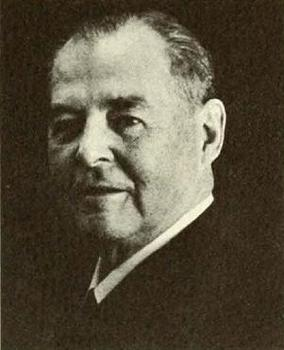
\includegraphics{images/hotelling.jpg}

}

\caption{Harold Hotelling}

\end{figure}
\end{column}

\begin{column}{0.48\textwidth}
The game I've described here is a version of a model originally
described by Harold Hotelling (1895-1973)
\end{column}
\end{columns}
\end{frame}

\begin{frame}{Feature Space}
\protect\hypertarget{feature-space}{}
\begin{itemize}[<+->]
\tightlist
\item
  Hotelling was less interested in physical location than location in
  feature space.
\item
  He wanted an explanation of why the products of competing firms tended
  to be like one another.
\end{itemize}
\end{frame}

\begin{frame}{Political Versions}
\protect\hypertarget{political-versions}{}
\begin{itemize}[<+->]
\tightlist
\item
  Games like this have become favorite tools of political scientists,
  arguing why political parties tended (at least in the 20th century!)
  to move towards the median.
\item
  You have to be careful about the payoffs here; political parties don't
  want to maximise votes, they want to maximise win probability and
  policy outcomes.
\item
  It turns out under a lot of assumptions you still get something like
  Hotelling's result, though it is sensitive to a lot of factors.
\end{itemize}
\end{frame}

\begin{frame}{Rationality Assumptions}
\protect\hypertarget{rationality-assumptions}{}
\begin{itemize}[<+->]
\tightlist
\item
  Finally, I want to briefly flag the rationality assumptions this
  argument needs.
\item
  As long as the players are rational, they won't play 0/6.
\item
  As long as they know the other player is rational, they won't play
  1/5.
\end{itemize}
\end{frame}

\begin{frame}{Rationality Assumptions}
\protect\hypertarget{rationality-assumptions-1}{}
\begin{itemize}[<+->]
\tightlist
\item
  But to rule out 2/4, we need something stronger. We need that they
  each know that the other knows that each is rational.
\item
  For longer beaches, we need even stronger assumptions. And those
  assumptions may be implausible.
\end{itemize}
\end{frame}

\hypertarget{nash-equilibrium}{%
\section{Nash Equilibrium}\label{nash-equilibrium}}

\begin{frame}{John Nash}
\protect\hypertarget{john-nash}{}
\begin{columns}[c]
\begin{column}{0.48\textwidth}
\begin{figure}

{\centering 
\includegraphics[width=0.75\textwidth,height=0.75\textheight]{images/crowe.png}

}

\caption{John Nash (via Hollywood)}

\end{figure}
\end{column}

\begin{column}{0.48\textwidth}
\begin{itemize}[<+->]
\tightlist
\item
  Nash Equilibrium is named after the American mathematician John Nash.
\item
  Except I seem to have a picture of Russell Crowe here.
\end{itemize}
\end{column}
\end{columns}
\end{frame}

\begin{frame}{John Nash}
\protect\hypertarget{john-nash-1}{}
\begin{columns}[c]
\begin{column}{0.48\textwidth}
\begin{figure}

{\centering 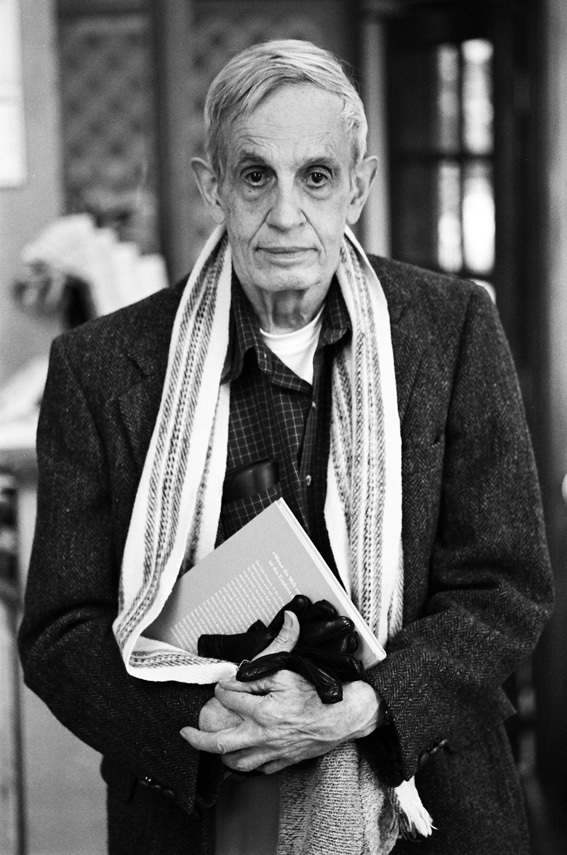
\includegraphics[width=0.75\textwidth,height=0.75\textheight]{images/nash.jpg}

}

\caption{John Nash}

\end{figure}
\end{column}

\begin{column}{0.48\textwidth}
\begin{itemize}[<+->]
\tightlist
\item
  Nash Equilibrium is named after the American mathematician John Nash
  (1928-2015).
\item
  It is the core concept of contemporary game theory.
\end{itemize}
\end{column}
\end{columns}
\end{frame}

\begin{frame}{Best Response}
\protect\hypertarget{best-response}{}
\begin{itemize}[<+->]
\tightlist
\item
  We will build up to it in stages.
\item
  The first important notion is that of a best response.
\item
  Strategy \(S\) is a best response to strategies by the other players
  iff no other strategy can do better, given what the other players are
  doing.
\end{itemize}
\end{frame}

\begin{frame}[plain]{}
\protect\hypertarget{section-9}{}
\begin{columns}[T]
\begin{column}{0.5\textwidth}
\begin{table}[!h]
\centering
\begin{tabular}[t]{>{}r|ccc}
\toprule
 & Left & Center & Right\\
\midrule
Up & 4, 3 & 2, 0 & 0, 5\\
Middle & 6, 2 & 0, 4 & 3, 1\\
Down & 3, 0 & 2, 1 & 4, 2\\
\bottomrule
\end{tabular}
\end{table}
\end{column}

\begin{column}{0.5\textwidth}
\begin{itemize}[<+->]
\tightlist
\item
  If Column plays Left, the best Row can do is play Middle.
\item
  They get 6 that way, and 3 or 4 from other plays.
\item
  So Middle is the best response to Left.
\end{itemize}
\end{column}
\end{columns}
\end{frame}

\begin{frame}[plain]{}
\protect\hypertarget{section-10}{}
\begin{table}[!h]
\centering
\begin{tabular}[t]{>{}r|ccc}
\toprule
 & Left & Center & Right\\
\midrule
Up & 4, 3 & 2, 0 & 0, 5\\
Middle & \fbox{6},2 & 0, 4 & 3, 1\\
Down & 3, 0 & 2, 1 & 4, 2\\
\bottomrule
\end{tabular}
\end{table}

\begin{itemize}[<+->]
\tightlist
\item
  We will represent the fact that it is a best response by putting a box
  around the payout.
\item
  There are all sorts of notations you'll see used for this; we'll just
  use a box.
\end{itemize}
\end{frame}

\begin{frame}[plain]{}
\protect\hypertarget{section-11}{}
\begin{table}[!h]
\centering
\begin{tabular}[t]{>{}r|ccc}
\toprule
 & Left & Center & Right\\
\midrule
Up & 4, 3 & 2, 0 & 0, 5\\
Middle & \fbox{6},2 & 0, 4 & 3, 1\\
Down & 3, 0 & 2, 1 & \fbox{4},2\\
\bottomrule
\end{tabular}
\end{table}

\begin{itemize}[<+->]
\tightlist
\item
  If Column plays Right, the best Row can do is play Down.
\item
  So we'll put a Box around it as well.
\end{itemize}
\end{frame}

\begin{frame}[plain]{}
\protect\hypertarget{section-12}{}
\begin{table}[!h]
\centering
\begin{tabular}[t]{>{}r|ccc}
\toprule
 & Left & Center & Right\\
\midrule
Up & 4, 3 & \fbox{2},0 & 0, 5\\
Middle & \fbox{6},2 & 0, 4 & 3, 1\\
Down & 3, 0 & \fbox{2},1 & \fbox{4},2\\
\bottomrule
\end{tabular}
\end{table}

\begin{itemize}[<+->]
\tightlist
\item
  Now if Column plays Middle, Row has two options that are tied for
  best: Top and Bottom.
\item
  They are both best responses.
\item
  So we'll put boxes around each.
\end{itemize}
\end{frame}

\begin{frame}[plain]{}
\protect\hypertarget{section-13}{}
\begin{table}[!h]
\centering
\begin{tabular}[t]{>{}r|ccc}
\toprule
 & Left & Center & Right\\
\midrule
Up & 4, 3 & \fbox{2},0 & 0,\fbox{5}\\
Middle & \fbox{6},2 & 0, 4 & 3, 1\\
Down & 3, 0 & \fbox{2},1 & \fbox{4},2\\
\bottomrule
\end{tabular}
\end{table}

\begin{itemize}[<+->]
\tightlist
\item
  I find it a little trickier to keep track of the best responses for
  Column, so I have to go a little slower.
\item
  If Row plays Top, Column has a choice of 3 (if they play Left), 0 (if
  they play Middle), or 5 (if they play Right).
\item
  5 is best, so the best response is Right.
\end{itemize}
\end{frame}

\begin{frame}[plain]{}
\protect\hypertarget{section-14}{}
\begin{table}[!h]
\centering
\begin{tabular}[t]{>{}r|ccc}
\toprule
 & Left & Center & Right\\
\midrule
Up & 4, 3 & \fbox{2},0 & 0,\fbox{5}\\
Middle & \fbox{6},2 & 0,\fbox{4} & 3, 1\\
Down & 3, 0 & \fbox{2},1 & \fbox{4},2\\
\bottomrule
\end{tabular}
\end{table}

\begin{itemize}[<+->]
\tightlist
\item
  If Row plays Middle, Column has a choice of 2 (if they play Left), 4
  (if they play Middle), or 1 (if they play Right).
\item
  4 is best, so the best response is Middle.
\end{itemize}
\end{frame}

\begin{frame}[plain]{}
\protect\hypertarget{section-15}{}
\begin{table}[!h]
\centering
\begin{tabular}[t]{>{}r|ccc}
\toprule
 & Left & Center & Right\\
\midrule
Up & 4, 3 & \fbox{2},0 & 0,\fbox{5}\\
Middle & \fbox{6},2 & 0,\fbox{4} & 3, 1\\
Down & 3, 0 & \fbox{2},1 & \fbox{4}, \fbox{2}\\
\bottomrule
\end{tabular}
\end{table}

\begin{itemize}[<+->]
\tightlist
\item
  If Row plays Down, Column has a choice of 0 (if they play Left), 1 (if
  they play Middle), or 2 (if they play Right).
\item
  2 is best, so the best response is Right.
\item
  We've now labelled all the (pure strategy) best responses.
\end{itemize}
\end{frame}

\begin{frame}{Nash Equilibrium}
\protect\hypertarget{nash-equilibrium-1}{}
\begin{itemize}[<+->]
\tightlist
\item
  A strategy set for all the players is a Nash Equilibrium if each
  player is making a best response to what the others are doing.
\item
  In these games, that means that both payoffs in the cell are boxed.
\end{itemize}
\end{frame}

\begin{frame}{Nash Equilibrium}
\protect\hypertarget{nash-equilibrium-2}{}
\begin{columns}[T]
\begin{column}{0.5\textwidth}
\begin{table}[!h]
\centering
\begin{tabular}[t]{>{}r|ccc}
\toprule
 & Left & Center & Right\\
\midrule
Up & 4, 3 & \fbox{2},0 & 0,\fbox{5}\\
Middle & \fbox{6},2 & 0,\fbox{4} & 3, 1\\
Down & 3, 0 & \fbox{2},1 & \fbox{4}, \fbox{2}\\
\bottomrule
\end{tabular}
\end{table}
\end{column}

\begin{column}{0.5\textwidth}
\begin{itemize}[<+->]
\tightlist
\item
  In this game, the unique Nash Equilibrium is Row plays Down, and
  Column plays Right.
\item
  That's the only cell where both players are making a best response to
  the other players' strategy.
\end{itemize}
\end{column}
\end{columns}
\end{frame}

\begin{frame}{Nash Equilibrium}
\protect\hypertarget{nash-equilibrium-3}{}
\begin{itemize}[<+->]
\tightlist
\item
  The general idea is that some strategies form an equilibrium if no one
  could do better by unilaterally changing strategy.
\item
  It's possible that players could do better if they both simultaneously
  changed - and we'll spend some time on cases where that happens.
\item
  But everyone is doing as well as they can given what everyone else is
  doing.
\end{itemize}
\end{frame}

\hypertarget{nash-equilibrium-and-philosophy}{%
\section{Nash Equilibrium and
Philosophy}\label{nash-equilibrium-and-philosophy}}

\begin{frame}{A Philosophical Claim}
\protect\hypertarget{a-philosophical-claim}{}
In any game where it is common knowledge that all the players are
rational, every player will play a strategy that forms part of a Nash
Equilibrium.
\end{frame}

\begin{frame}{Status of Nash}
\protect\hypertarget{status-of-nash}{}
\begin{itemize}[<+->]
\tightlist
\item
  I think most economists and political scientists accept something like
  this.
\item
  But I think philosophers who work on game theory more often do not
  accept it.
\end{itemize}
\end{frame}

\begin{frame}{Arguments for Nash}
\protect\hypertarget{arguments-for-nash}{}
\begin{itemize}[<+->]
\tightlist
\item
  Oddly, it's hard to find canonical arguments for the importance of
  Nash.
\item
  It's so deeply embedded in game theory that it doesn't get discussed
  in research articles, more in textbooks.
\item
  Bonanno has a passage on page 40 that you could (perhaps uncharitably)
  count as a contribution to that genre.
\end{itemize}
\end{frame}

\begin{frame}{Transparency of Reason Interpretation}
\protect\hypertarget{transparency-of-reason-interpretation}{}
\begin{quote}
If players are all ``equally rational'' and Player 2 reaches the
conclusion that she should play y, then Player 1 must be able to
duplicate Player 2's reasoning process and come to the same conclusion;
it follows that Player 1's choice of strategy is not rational unless it
is a strategy x that is optimal against y. A similar argument applies to
Player 2's choice of strategy (y must be optimal against x) and thus
(x,y) is a Nash equilibrium.
\end{quote}
\end{frame}

\begin{frame}{Transparency of Reason Interpretation}
\protect\hypertarget{transparency-of-reason-interpretation-1}{}
\begin{itemize}[<+->]
\tightlist
\item
  This doesn't look like a good argument for the Philosophical Claim.
\item
  All it shows is the weaker claim that if there is a uniquely rational
  play for each player, those plays will form a Nash Equilibrium.
\end{itemize}
\end{frame}

\begin{frame}{Viable recommendation interpretation}
\protect\hypertarget{viable-recommendation-interpretation}{}
\begin{quote}
Imagine that a third party makes a public recommendation to each player
on what strategy to play; then no player will have an incentive to
deviate from the recommendation (if she believes that the other players
will follow the recommendation) if and only if the recommended strategy
profile is a Nash equilibrium.
\end{quote}
\end{frame}

\begin{frame}{Viable recommendation interpretation}
\protect\hypertarget{viable-recommendation-interpretation-1}{}
\begin{itemize}[<+->]
\tightlist
\item
  Again, this argument only works if the third party makes a unique
  recommendation.
\item
  If the third party says ``Do one of these three things'', there is no
  argument that all three have to be Nash.
\end{itemize}
\end{frame}

\begin{frame}{Self-enforcing agreement interpretation}
\protect\hypertarget{self-enforcing-agreement-interpretation}{}
\begin{quote}
Imagine that the players are able to communicate before playing the game
and reach a non-binding agreement expressed as a strategy profile s;
then no player will have an incentive to deviate from the agreement (if
she believes that the other player will follow the agreement) if and
only if s is a Nash equilibrium.
\end{quote}
\end{frame}

\begin{frame}{Self-enforcing agreement interpretation}
\protect\hypertarget{self-enforcing-agreement-interpretation-1}{}
\begin{itemize}[<+->]
\tightlist
\item
  This is right as far as it goes, but doesn't help defend the
  philosophical claim in cases where no communication is possible.
\item
  And here it is particularly notable that Bonanno's purposes are not
  quite the same as mine.
\end{itemize}
\end{frame}

\begin{frame}{No regret interpretation}
\protect\hypertarget{no-regret-interpretation}{}
\begin{quote}
s is a Nash equilibrium if there is no player who, after observing the
opponent's choice, regrets his own choice (in the sense that he could
have done better with a different strategy of his, given the observed
strategy of the opponent).
\end{quote}

\begin{itemize}[<+->]
\tightlist
\item
  This is a very good clear definition of what Nash is, but hard to see
  how it's a an argument for the importance of Nash.
\end{itemize}
\end{frame}

\begin{frame}{Other Arguments}
\protect\hypertarget{other-arguments}{}
\begin{itemize}[<+->]
\tightlist
\item
  You might be being spied on.
\item
  The other player might be a mind-reader.
\item
  You might be playing repeatedly, and so your strategy will be (more or
  less) revealed.
\end{itemize}
\end{frame}

\begin{frame}{Repeated Games}
\protect\hypertarget{repeated-games}{}
\begin{itemize}[<+->]
\tightlist
\item
  The last one is, I think, the main reason in practice people care
  about Nash.
\item
  But it turns out for one important game, the Prisoners Dilemma, it is
  arguable that in the repeated game you should not play the Nash
  equilibrium.
\end{itemize}
\end{frame}

\begin{frame}{Prisoners' Dilemma}
\protect\hypertarget{prisoners-dilemma}{}
\begin{columns}[T]
\begin{column}{0.4\textwidth}
\begin{table}[!h]
\centering
\begin{tabular}[t]{>{}r|cc}
\toprule
 & Coop & Defect\\
\midrule
Coop & 3, 3 & 0, \fbox{5}\\
Defect & \fbox{5}, 0 & \fbox{1}, \fbox{1}\\
\bottomrule
\end{tabular}
\end{table}
\end{column}

\begin{column}{0.6\textwidth}
\begin{itemize}[<+->]
\tightlist
\item
  The only Nash equilibrium is both players defect.
\item
  And personally, I think in the one-shot game they should both defect.
\item
  But it is not at all obvious they should defect in the repeated game.
\item
  We will return to this point a lot in a few weeks.
\end{itemize}
\end{column}
\end{columns}
\end{frame}

\begin{frame}{For Next Week}
\protect\hypertarget{for-next-week}{}
\begin{itemize}[<+->]
\tightlist
\item
  We will start looking at chapter 3, on games that have sequential
  moves.
\end{itemize}
\end{frame}



\end{document}
